% !TEX root = /home/maa/dev/PHD/docs/paper5/main.tex
%% 
%% Copyright 2007-2020 Elsevier Ltd
%% 
%% This file is part of the 'Elsarticle Bundle'.
%% ---------------------------------------------
%% 
%% It may be distributed under the conditions of the LaTeX Project Public
%% License, either version 1.2 of this license or (at your option) any
%% later version.  The latest version of this license is in
%%    http://www.latex-project.org/lppl.txt
%% and version 1.2 or later is part of all distributions of LaTeX
%% version 1999/12/01 or later.
%% 
%% The list of all files belonging to the 'Elsarticle Bundle' is
%% given in the file `manifest.txt'.
%% 
%% Template article for Elsevier's document class `elsarticle'
%% with harvard style bibliographic references

%\documentclass[preprint,12pt,authoryear]{elsarticle}
\documentclass[preprint,9pt,authoryear]{elsarticle}

%% Use the option review to obtain double line spacing
%%\documentclass[authoryear,preprint,review,12pt]{elsarticle}

%% Use the options 1p,twocolumn; 3p; 3p,twocolumn; 5p; or 5p,twocolumn
%% for a journal layout:
%% \documentclass[final,1p,times,authoryear]{elsarticle}
%%\documentclass[final,1p,times,twocolumn,authoryear]{elsarticle}
%% \documentclass[final,3p,times,authoryear]{elsarticle}
%% \documentclass[final,3p,times,twocolumn,authoryear]{elsarticle}
%% \documentclass[final,5p,times,authoryear]{elsarticle}
%%\documentclass[final,5p,times,twocolumn,authoryear]{elsarticle}

%% For including figures, graphicx.sty has been loaded in
%% elsarticle.cls. If you prefer to use the old commands
%% please give \usepackage{epsfig}

%% The amssymb package provides various useful mathematical symbols
\usepackage{amssymb}
%% The amsthm package provides extended theorem environments
%% \usepackage{amsthm}

%% The lineno packages adds line numbers. Start line numbering with
%% \begin{linenumbers}, end it with \end{linenumbers}. Or switch it on
%% for the whole article with \linenumbers.
%% \usepackage{lineno}
\usepackage{amsmath}
\usepackage{pgfplotstable,filecontents}
\usepackage{hyperref}
\usepackage{amsmath}
\usepackage{placeins}  % for \FloatBarrier
\usepackage{svg}
\usepackage{caption}
\usepackage{subcaption}
%\usepackage{cancel}
\usepackage{flafter}  % no figures before reference
%\usepackage{layouts}
\usepackage{bm}  % bold text

\journal{International Journal of Naval Architecture and Ocean Engineering}

\begin{document}

\begin{frontmatter}

    %% Title, authors and addresses

    %% use the tnoteref command within \title for footnotes;
    %% use the tnotetext command for theassociated footnote;
    %% use the fnref command within \author or \affiliation for footnotes;
    %% use the fntext command for theassociated footnote;
    %% use the corref command within \author for corresponding author footnotes;
    %% use the cortext command for theassociated footnote;
    %% use the ead command for the email address,
    %% and the form \ead[url] for the home page:
    %% \title{Title\tnoteref{label1}}
    %% \tnotetext[label1]{}
    %% \author{Name\corref{cor1}\fnref{label2}}
    %% \ead{email address}
    %% \ead[url]{home page}
    %% \fntext[label2]{}
    %% \cortext[cor1]{}
    %% \affiliation{organization={},
    %%            addressline={}, 
    %%            city={},
    %%            postcode={}, 
    %%            state={},
    %%            country={}}
    %% \fntext[label3]{}

    %\title{System identification of a physics-informed ship model for better predictions in wind conditions}
    %\title{Virtual Captive Tests for Identifying System-Based Manoeuvring Models}
    \title{Identification of manoeuvring models for wind-assisted ships with large rudders using virtual captive tests}
    

    %% use optional labels to link authors explicitly to addresses:
    %% \author[label1,label2]{}
    %% \affiliation[label1]{organization={},
    %%             addressline={},
    %%             city={},
    %%             postcode={},
    %%             state={},
    %%             country={}}
    %%
    %% \affiliation[label2]{organization={},
    %%             addressline={},
    %%             city={},
    %%             postcode={},
    %%             state={},
    %%             country={}}

    \author[1,2]{Martin Alexandersson\corref{cor1}%
        %\fnref{fn1,fn3}
    }
    \ead{maralex@chalmers.se}
    \author[1]{Wengang Mao}
    \author[1]{Jonas W. Ringsberg}
    \author[2]{Martin Kjellberg}


    \affiliation[1]{organization={Dept. of Mechanics and Maritime Sciences, Division of Marine Technology, Chalmers University of Technology},%Department and Organization
        addressline={Hörsalsvägen 7A},
        city={Gothenburg},
        postcode={41296},
        country={Sweden}}


    \affiliation[2]{organization={Research Institutes of Sweden (RISE), SSPA Maritime Center},%Department and Organization
        addressline={Chalmers tvärgata 10},
        city={Gothenburg},
        postcode={41296},
        country={Sweden}}

    \cortext[cor1]{Corresponding author}

    \begin{abstract}
        % Move 1 - Background/introduction/situation 
Ships with wind-assisted propulsion systems (WAPS) are often equipped with large rudders to compensate for WAPS-induced drifting forces. The WAPS also significantly affects the effectiveness of mathematical models used to describe the ship's manoeuvring characteristics. In this study, a modular manoeuvring model is proposed to enhance the original MMG model, aiming to produce accurate manoeuvring simulations for ships with WAPS.

% Move 3 - Methods/materials/subjects/procedures 
Methods of virtual captive tests (VCT) are proposed to recreate the forces acting on WAPS ships during free-running model tests (FRMT) in motor mode, identifying all the parameters in the modular model. The hydrodynamic damping coefficients within the model are determined through linear regression of the VCT data. The added masses are then determined from pure yaw and pure sway simulations using a fully nonlinear potential flow (FNPF) panel method.

% Move 4 - Results/findings 
Two ships designed for WAPS, wPCC and Optiwise, are used to validate the proposed method based on the inverse dynamics of their experimental model tests. The wPCC is equipped with a semi-empirical rudder that has previously shown to work well for this twin-rudder ship. The Optiwise single rudder is modeled with a new quadratic version of the MMG rudder model, proposed in this paper. It is concluded that inverse dynamics analysis, together with state VCTs, is an efficient way to analyze the models, and the manoeuvring model can be efficiently identified when correct VCTs are used in the proposed method. However, the inverse dynamics analysis also revealed potential errors in the wPCC VCT data due to false assumptions about wave generation and roll motion. The Optiwise test case, where these assumptions should be more valid, showed much better agreement with the FRMT inverse dynamics.

% Move 5 - Discussion/conclusion/significance
%This paper has proposed a new version of the MMG model that produced accurate simulations when identified on correct VCT data. .

%    

%For the wPCC ship with double rudders, large discrepancies were observed between the closed loop manoeuvring predictions by the identified model and tests, due to the incapability of VCTs to model rudder forces, and asymmetric patterns of flows on the two rudders. When the measurement of rudder forces is available for the Optiwise ship, the MMG model identified by the proposed method can perfectly predict the ship’s manoeuvring motions compared to the tests.


    \end{abstract}

    %%Graphical abstract
    %\begin{graphicalabstract}
    %    %\includegraphics{grabs}
    %\end{graphicalabstract}
    %
    %%%Research highlights
    %\begin{highlights}
    %    \item Research highlight 1
    %    \item Research highlight 2
    %\end{highlights}

    \begin{keyword}
    Inverse dynamics \sep Physics-informed maneuvering model \sep System identification \sep Wind-assisted propulsion 
        %% keywords here, in the form: keyword \sep keyword

        %% PACS codes here, in the form: \PACS code \sep code

        %% MSC codes here, in the form: \MSC code \sep code
        %% or \MSC[2008] code \sep code (2000 is the default)

    \end{keyword}

\end{frontmatter}
%% \linenumbers
%textwidth in inches: \printinunitsof{in}\prntlen{\textwidth} \newline
%textheight in inches: \printinunitsof{in}\prntlen{\textheight}
%% main text
%\newpage
\section*{Nomenclature}
\label{sec:introduction}
\begin{table}[h]
    \centering
    %\footnotesize
    \scriptsize
    %\caption{Semi-empirical rudder parameters (SI units) in model scale.}
    \label{tab:other_parameters}
    \pgfplotstabletypeset[col sep=comma, column type=r,
    columns/LaTeX/.style={column type=r,string type,column name=~},
    columns/LaTeX1/.style={column type=r,string type, column name=~},
    columns/LaTeX2/.style={column type=r,string type, column name=~},
    %columns/LaTeX3/.style={column type=l,string type, column name=~},
    columns/Description/.style={column type=p{3.3cm},string type,column name=~},
    columns/Description1/.style={column type=p{3.3cm},string type, column name=~},
    columns/Description2/.style={column type=p{3.3cm},string type, column name=~},
    %columns/Description3/.style={column type=l,string type, column name=~},
    %every head row/.style={before row=\hline,after row=\hline},
    %every last row/.style={after row=\hline}
    ]{tables/mathematical_model_kinetics.nomenclature.csv}
\end{table}
\FloatBarrier

\section*{Abbreviations}
\label{sec:introduction}
\begin{table}[h]
    \centering
    %\footnotesize
    \scriptsize
    %\caption{Semi-empirical rudder parameters (SI units) in model scale.}
    \label{tab:abbreviations}
    \begin{tabular}{l l}

    CFD & Computational fluid dynamics \\
    CMT & Captive model tests \\
    DOF & Degree of freedom \\
    FRMT & Free running model tests \\
    ID & Inverse dynamics \\
    MMG & Manoeuvring modeling group \\
    OLS & Ordinary least-square \\
    RHI & Rudder hull interaction \\
    RISE & Research institutes of Sweden \\
    VCT & Virtual captive tests \\
    WASP & wind-assisted ship propulsion \\
    wPCC & Wind powered car carrier test case\\
    \end{tabular}
        
\end{table}
\FloatBarrier

%%%%%%%%%%%%%%%
%% INTRODUCTION
%%%%%%%%%%%%%%%
\section{Introduction}
\label{sec:introduction}
Ships greater than 100 meters must meet maneuverability requirements to ensure navigation safety \citep{imoStandardsShipManoeuvrability2002}. As the urgent demands to decarbonize the shipping industry increase, wind-assisted propulsion systems (WAPS) can become essential equipment on future ships \citep{nelissenStudyAnalysisMarket2016}. Ships with WAPS are often equipped with large rudders to compensate for significant side forces.

The maneuvering characteristics of a ship can be predicted using various approaches. The possibilities differ significantly between an existing ship, where operational data is available, and a new ship, where no operational data is yet available. The data can be categorized as either free running test (FT) data, where the ship is exposed to forces (the input) and resulting trajectories are recorded (the output), or the reversed scenario in captive test (CT) data, where the trajectory is the input and resulting forces are the output. FT data can be collected for existing ships, but also for new ships in free-running model tests, which are often recognized as the most reliable way to predict a ship's maneuverability \citep{ittcITTCRecommendedProcedures2008}. FT data can also be collected from direct CFD calculations at full scale, avoiding the scale effects of model tests. Regardless of the method used to obtain FT data, it only describes the maneuvering characteristics for a set of preset and often standardized maneuvers \citep{imoStandardsShipManoeuvrability2002} that do not generalize to other speeds or maneuvers, which can be a drawback of this approach. However, generalized results can be obtained with system identification, where a prediction model can be identified from the FT data as described by \citet{luoParameterIdentificationShip2016, xuUncertaintyAnalysisHydrodynamic2019, wangOptimalDesignExcitation2020, alexanderssonSystemIdentificationVessel2022, haoRecurrentNeuralNetworks2022a, kimValidation4DOFManeuvering2024, alexanderssonSystemIdentificationPhysicsinformed2024b}.

Most ship designs with WAPS are new building projects, where the ship does not yet exist, so the maneuvering characteristics must be studied by model tests or CFD calculations. Free running tests can be conducted with CFD \citep{sakamotoURANSSimulationsStatic2012, elmoctarRANSBasedSimulatedShip2014, dumanTurnZigzagManoeuvres2022}. However, if high accuracy is required, this might be a computationally expensive option in most cases. A more efficient approach is to conduct captive tests with CFD in virtual captive tests (VCT) as input to a system-based prediction model that can simulate the desired maneuvers as described by \citet{simonsenKCSPMMTests2014, elmoctarRANSBasedSimulatedShip2014, hajivandVirtualSimulationManeuvering2015, yoonBenchmarkCFDValidation2015c, liuPredictionsShipManeuverability2018}. These CFD-based methods were used to simulate very complicated navigation scenarios even without extensive model test experience, such as free-running ship movements in following waves \citep{Araki2019}, the hull-propulsor-engine interaction during maneuvering of a ship \citep{elmoctarRANSBasedSimulatedShip2014}, and turn and zigzag maneuvers for catamarans \citep{dumanTurnZigzagManoeuvres2022}.

For conventional ships, different mathematical models to describe their maneuverability have been well investigated, while empirical formulas are available for some maneuvering components \citep{yasukawaIntroductionMMGStandard2015}. For ships with WAPS installed, ship maneuverability can be significantly affected due to extra WAPS and large rudders, which can cause different flow characteristics for propeller-rudder interactions and obvious drifting. 



There is a lack of experience on how their maneuverability should be modeled. In this study, a systematic approach is proposed to obtain hydrodynamic coefficients and hydrodynamic derivatives in an MMG-style model, as well as modeling of rudder forces under various drifting conditions. Cost-effective CFD-based virtual captive tests are proposed to obtain some necessary parameters in the MMG model. In this study, two ships designed with WAPS and different propulsion settings are used to validate the proposed approach.

For a complete description of the proposed method, the remaining part of the paper is organized as follows. The maneuvering model is first introduced in \autoref{sec:model}. The two test cases are presented in \autoref{sec:test_cases} together with the method to preprocess the experimental data and how the inertia of the ships was determined. The proposed method for parameter identification is introduced in \autoref{sec:PIT}. The results are presented in \autoref{sec:results_wpcc} for wPCC and in \autoref{sec:results_optiwise} for Optiwise, followed by the study conclusions in \autoref{sec:conclusions}.


%A ship is a system that transports passengers and goods on water. Manoeuvring, is a fundamental aspect of this system. The ability to control the ship from departure to destination along a desired route, avoiding obstacles such as land and other ships is an essential. The IMO standards for manoeuvrability highlights the importance of the ship manoeuvring. The performance can be assessed by conducting standard manoeuvres with the real built system – the ship, during sea trials. Revealing a substandard manoeuvring performance at this stage is however undesirable, where the possibilities for design changes are very limited and costly. This calls for earlier assessments, before the ship is build, which is traditionally done in scale model tests with a free sailing model.

%With the advancement of numerical methods, CFD is an alternative, which may be more cost efficient and potentially more accurate, where the scale effect problem can be avoided by conducting full scale simulations. Direct CFD calculations in the time domain, visiting all the states during a manoeuvre, are however computationally expensive, even more expensive than the scale model tests and is therefore mostly applied in a research context, than in commercial ship building projects.

%Virtual captive tests (VCT) can be used to reduce the computational effort by only calculating a few potential states of a manoeuvre with CFD. The calculated forces acting on the ship for the sampled states can be used to develop a prediction model, which can be used to simulate the unseen states during the manoeuvre.  

%The CFD calculations for the VCT in this paper are assumed to have sufficient accuracy. The accuracy of the CFD itself will therefore not be questioned. Instead, the accuracy of the hydrodynamic discretization in developing a system based model from a set of VCT is the main focus.  

%%%%%%%%%%%%%%%
%% MODEL
%%%%%%%%%%%%%%%
\section{Model}
\noindent The ship manoeuvring dynamics is modeled as a state space model (\autoref{eq:state_space})
\begin{equation}
    \dot{\mathbf{x}}=f(\mathbf{x},\mathbf{u})
    \label{eq:state_space}
\end{equation}
where the change of state $\dot{\mathbf{x}}$ is expressed as function of the current state vector $\mathbf{x}$ and the input vector $\mathbf{u}$ through the transition function $f(\mathbf{x},\mathbf{u})$. A state with the position and orientation, velocities and turning rate defines the state of the ship in 3 DOF (\autoref{eq:state}). 
\begin{equation}
    \mathbf{x} = [x0,y0,\Psi, u,v,r]^T
    \label{eq:state}
\end{equation}

\subsection{Prime system}
\label{sec:prime_system}
\noindent Some variables in the equations are expressed as non-dimensional units using the prime system, denoted by the prime symbol ($'$). Variables are converted from SI units to the prime system using the denominators in \autoref{tab:prime_system} for the corresponding physical quantity, where $U$ and $L$ are the velocity and length between the perpendiculars of the ship, respectively, and $\rho$ is the water density.
For the calculation of surge velocity $u'$, the perturbed velocity $(u-U_0)$ about a nominal speed $U_0$ is used, as in \autoref{eq:u_prime}, to avoid a $u'$ of 1 for all speeds when the ship is on a straight course (where $u=U$), as in a resistance or self-propulsion test, 
\begin{equation}
    \label{eq:u_prime}
    u' = \frac{u-U_0}{U}, \hspace{0.1cm}
    F_{n0} = \frac{U_0}{\sqrt{g \cdot L}}
\end{equation}
where $U_0$ is instead expressed as a Froude number for a non-dimensional variable.
% \begin{equation}
%     \label{eq:Fn0}
%     F_{n0} = \frac{U_0}{\sqrt{g \cdot L}}
% \end{equation}
The usage of the perturbed velocity, therefore, allows for higher order resistance terms in the model, such as $X_{u}$, which are otherwise not possible. 
\begin{table}[h]
    \caption{Scalings used in the prime system.}
    \label{tab:prime_system}
    \centering
    \pgfplotstabletypeset[col sep=comma,
        columns={Physical quantity, SI unit, Denominator},
        columns/SI unit/.style={string type},
        columns/Physical quantity/.style={string type},
        columns/Denominator/.style={string type},
        column type=l,	% specify the align method
        every head row/.style={before row=\hline,after row=\hline},	% style the first row
        every last row/.style={after row=\hline},	% style the last row
    ]{tables/prime_system.prime_system_short.csv}
\end{table}
\FloatBarrier
\subsection{Hull model}
\noindent Based on the above-mentioned prime system, the hydrodynamic forces acting on a ship's hull as in Eq.(\ref{eq:X_D}) can be described viz,
\begin{equation}
    \label{eq:XYN_H}
    \left.\begin{aligned}
    X_H & = 1/2\rho L^{2} U^{2} X_H^{'}  \\
    Y_H & = 1/2\rho L^{2} U^{2} Y_H^{'}  \\
    N_H & = 1/2\rho L^{3} U^{2} X_H^{'}
    \end{aligned}\right\}
\end{equation}
where the non-dimensional surge force $X_H^{'}$, lateral force $Y_H^{'}$ and yaw moment $N_H^{'}$ are normally modeled by the following general polynomials in terms of non-dimensional velocities $u^{'}, v^{'}$ and yaw rate $r'$ based on the MMG model, \citep{yasukawaIntroductionMMGStandard2015},
\begin{equation}
    \label{eq:XYN_H_prime}
    \left.\begin{aligned}
    \input{equations/mathematical_model_kinetics.X_H} \\
    \input{equations/mathematical_model_kinetics.Y_H} \\
    \input{equations/mathematical_model_kinetics.N_H}
    \end{aligned}\right\}
\end{equation}
where the coefficients $X_0^{'}, X_{rr}^{'}, X_u^{'}, X_{vr}^{'}, X_{vv}^{'}, Y_{0}^{'}, Y_{rrr}^{'}, Y_{r}^{'}, Y_{vrr}^{'}, Y_{vvr}^{'}, Y_{vvv}^{'}, Y_{v}^{'}, N_{0}^{'}$, $N_{rrr}^{'}$, $N_{r}^{'}$, $N_{vrr}^{'}$, $N_{vvr}^{'}$, $N_{vvv}^{'}$, $N_{v}^{'}$ are referred as the hydrodynamic derivatives on ship maneuvering, and they represent the impact of different velocity components to the three hydrodynamic forces on the ship's hull. An important task for system identification of ship maneuvering in this study is to find those derivatives.

In this study, the perturbed surge velocity is proposed to allow for the extra resistance term ${X_u}'$, so that the resistance curve does not need to have a quadratic shape as in the MMG model.  
%
% \begin{equation}
%     \label{eq:Y_H}
%     \input{equations/mathematical_model_kinetics.Y_H}
% \end{equation}
% %
% \begin{equation}
%     \label{eq:N_H}
%     \input{equations/mathematical_model_kinetics.N_H}
% \end{equation}
\subsection{Rudder models}
A modified quadratic MMG rudder model has been proposed as an enhancement tot he original MMG rudder model \citep{yasukawaIntroductionMMGStandard2015}.




%%%%%%%%%%%%%%%
%% METHODOLOGY
%%%%%%%%%%%%%%%
\section{Methodology}
\subsection{Test cases}
\noindent Two test models/cases have been studied in this paper, named as wPCC and Optiwise. The wPCC test case is the ship model that was designed for wind-assisted propulsion systems (WAPS) and can alter between a fully sailing mode, and a fully motoring mode, and in between. 
However, this paper only considers the motoring mode. The wPCC design differs from conventional motoring cargo ship designs in that the ship has two very large rudders, they are actually two to three times larger than needed for a conventional ship. The ship also has fins at the bilge to generate extra lift while sailing, as shown on the scale model in \autoref{fig:wPCC}.
\autoref{tab:main_particulars} shows the main particulars of the scale model. 

\begin{figure}[h]
    \centering
    \includegraphics[width=\columnwidth]{figures/5m2.jpg}
    \caption{Scale model of the wPCC used in the model tests. Copyright RISE.}
    \label{fig:wPCC}
\end{figure}

The Optiwse test case is an ordinary VLCC tanker but with a larger rudder size adopted for WAPS as shown in the scale model in \autoref{fig:optiwise} with main particulars according to \autoref{tab:main_particulars}.
FRMTs with Optiwise were conducted as a continuation of the wPCC experiments, with a more conventional ship design. The experiments were run at a lower Froude number, compared to wPCC, so that wave generation and roll would have smaller impacts. The larger rudder was expected to play a more important part of the total hydrodynamics, compared to conventional ships. The model was therefore equipped with rudder force transducers, so that the rudder forces could be observed during the maneuvers. 
\begin{figure}[h]
    \centering
    \includegraphics[width=\columnwidth]{figures/optiwise.jpg}
    \caption{Scale model of the Optiwise used in the model tests. Copyright RISE.}
    \label{fig:optiwise}
\end{figure}
\begin{table}[h]
    \centering
    \caption{Main particulars (SI units) of the wPCC scale model.}
    \label{tab:main_particulars}
    \pgfplotstabletypeset[col sep=comma, column type=r,
        columns/Parameter/.style={column type=l,string type},
        columns/Unit/.style={column type=l,string type,column name=~},
        columns/Description/.style={column type=l,string type},
        columns/Value/.style={column type=r, column name=~},
        every head row/.style={before row=\hline,after row=\hline},
        every last row/.style={after row=\hline}
    ]{tables/test_cases.main_particulars.csv}
\end{table}
\FloatBarrier

\subsection{Inertia}
The mass properties of the ship, including the added masses, need to be determined in order to conduct simulations or inverse dynamics with the ship model. The rigid body mass and mass inertia were determined with swing tests in air before conducting the FMT at RISE MDL. The vertical centre of gravity (VCG) was determined with inclining experiments with the scale model in the MDL basin.

The yaw added mass $N_{\dot{r}}$ was determined with the Fourier series method \citep{sakamotoURANSSimulationsStatic2012} applied on a pure yaw test conducted in ShipFlow Motions \citep{kjellbergFullyNonlinearUnsteady2013}.
During the pure yaw test the heading $\Psi$ is varied according to \autoref{eq:pure_yaw_psi} so that the yaw rate $r$ and yaw acceleration $\dot{r}$ are varied according to \autoref{eq:pure_yaw_r}, and \autoref{eq:pure_yaw_r1d}.
\begin{equation}
    \Psi = - \Psi_{max} \cos{\left(t w \right)}
    \label{eq:pure_yaw_psi}
\end{equation}
\begin{equation}
    r = \Psi_{max} w \sin{\left(t w \right)}
    \label{eq:pure_yaw_r}
\end{equation}
\begin{equation}
    \dot{r} = \Psi_{max} w^{2} \cos{\left(t w \right)}
    \label{eq:pure_yaw_r1d}
\end{equation}


The sway added mass $Y_{\dot{v}}$ were determined in a similar way, but instead by conducting a pure sway test (see [[Pure sway test]]). The coupled added masses $N_{\dot{v}}$, and $Y_{\dot{r}}$ were determined with strip theory calculations using Franks close fit method.
%\subsection{VCT matrix for wPCC}
%\begin{table}[h]
    \centering
    \small
    \caption{VCT variations for wPCC.}
    \label{tab:inflow_to_rudder_force}
    \pgfplotstabletypeset[col sep=comma, column type=c, style=string type,
        columns/Test type/.style={column type=l,string type},
        columns/V/.style={column type=c,string type, column name=$V$ [m/s]},
        columns/beta_deg/.style={column type=c,string type, column name=$\beta$ [deg]},
        columns/r/.style={column type=c,string type, column name=$r$ [rad/s]},
        columns/delta_deg/.style={column type=c,string type, column name=$\delta$ [deg]},
        columns/rev/.style={column type=c,string type, column name=rev [1/s]},
        %columns/r/.style={column type=r,fixed,fixed zerofill,precision=2, column name=$r$ [rad/s]},
        %columns/V_R/.style={fixed,fixed zerofill,precision=2, column name=$V_R$ [m/s]},
        %columns/gamma_deg/.style={fixed,fixed zerofill,precision=1, column name=$\gamma$ [deg]},
        %columns/Y_R/.style={fixed,fixed zerofill,precision=1, column name=$Y_R^{VCT}$ [N]},
        %columns/Y_R_MMG/.style={fixed,fixed zerofill,precision=1, column name=$Y_R^{MMG}$ [N]},
        every head row/.style={before row=\hline,after row=\hline},
        every last row/.style={after row=\hline}
    ]{tables/methodology_VCT_wPCC.variations.csv}
\end{table}
\begin{figure}[h]
    \includesvg{figures/methodology_VCT_wPCC.phase_plot.svg}
    \caption{Phase plots of the wPCC zigzag tests together with the coverage of the VCTs and extra state VCTs.}
    \label{fig:VCT_phase_plot_wPCC}
\end{figure}
\subsection{Inverse dynamics analysis}
\subsection{state VCT}
\subsection{Hydrodynamic forces from VCT}
VCT calculations are conducted by solving a set of static flow calculations with CFD. The VCT test matrices (\autoref{tab:VCT_wPCC}, \autoref{tab:VCT_optiwise}) are selected to have a good coverage of the states that the ship will have during the maneuver. How the combinations of drift angle and yaw rate have been selected is shown in \autoref{fig:phase_plots}, for the wPCC and Optiwise. 
\begin{figure}[h]
     \centering
     \begin{subfigure}[b]{0.49\textwidth}
         \centering
         \includesvg{figures/methodology_VCT_wPCC.phase_plot.svg}
        \caption{wPCC.}
        \label{fig:VCT_phase_plot_wPCC}
     \end{subfigure}
     \hfill
     \begin{subfigure}[b]{0.49\textwidth}
        \centering
        \includesvg{figures/methodology_VCT_optiwise.phase_plot.svg}
        \caption{Optiwise.}
        \label{fig:VCT_phase_plot_optiwise}
     \end{subfigure}
        \caption{Phase plots of the zigzag tests together with the coverage of the VCTs and extra state VCTs.}
        \label{fig:phase_plots}
\end{figure}

The total forces from the VCT $X_{VCT}$, $Y_{VCT}$, and $N_{VCT}$ are recalculated with \autoref{eq:X_D} -- \autoref{eq:N_D}, to obtain the damping forces.
\begin{equation}
    \label{eq:X_D}
    X_{D} = X_{VCT} + Y_{\dot{r}} r^{2} + Y_{\dot{v}} r v
\end{equation}
\begin{equation}
    \label{eq:Y_D}
    Y_{D} = - X_{\dot{u}} r u + Y_{VCT}
\end{equation}
\begin{equation}
    \label{eq:N_D}
    N_{D} = N_{VCT} + X_{\dot{u}} u v - Y_{\dot{r}} r u - Y_{\dot{v}} u v
\end{equation}
The mass $m$ has disappeared from \autoref{eq:F_expanded} to arrive at these expressions, because the ship is not moving in ShipFlow, instead the water is having an either oblique or circular inflow \citep{roychoudhuryCFDSimulationsSteady2017}.
% wPCC
\begin{table}[h]
    \centering
    \small
    \caption{VCT variations for wPCC.}
    \label{tab:VCT_wPCC}
    \pgfplotstabletypeset[col sep=comma, column type=c, style=string type,
        columns/Test type/.style={column type=l,string type},
        columns/V/.style={column type=c,string type, column name=$V$ [m/s]},
        columns/beta_deg/.style={column type=c,string type, column name=$\beta$ [deg]},
        columns/r/.style={column type=c,string type, column name=$r$ [rad/s]},
        columns/delta_deg/.style={column type=c,string type, column name=$\delta$ [deg]},
        columns/rev/.style={column type=c,string type, column name=rev [1/s]},
        %columns/r/.style={column type=r,fixed,fixed zerofill,precision=2, column name=$r$ [rad/s]},
        %columns/V_R/.style={fixed,fixed zerofill,precision=2, column name=$V_R$ [m/s]},
        %columns/gamma_deg/.style={fixed,fixed zerofill,precision=1, column name=$\gamma$ [deg]},
        %columns/Y_R/.style={fixed,fixed zerofill,precision=1, column name=$Y_R^{VCT}$ [N]},
        %columns/Y_R_MMG/.style={fixed,fixed zerofill,precision=1, column name=$Y_R^{MMG}$ [N]},
        every head row/.style={before row=\hline,after row=\hline},
        every last row/.style={after row=\hline}
    ]{tables/methodology_VCT_wPCC.variations.csv}
\end{table}
%\begin{figure}[h]
%    \includesvg{figures/methodology_VCT_wPCC.phase_plot.svg}
%    \caption{Phase plots of the wPCC zigzag tests together with the coverage of the VCTs and extra state VCTs.}
%    \label{fig:VCT_phase_plot_wPCC}
%\end{figure}

% Optiwise
\begin{table}[h]
    \centering
    \small
    \caption{VCT variations for Optiwise.}
    \label{tab:VCT_optiwise}
    \pgfplotstabletypeset[col sep=comma, column type=c, style=string type,
        columns/Test type/.style={column type=l,string type},
        columns/V/.style={column type=c,string type, column name=$V$ [m/s]},
        columns/beta_deg/.style={column type=c,string type, column name=$\beta$ [deg]},
        columns/r/.style={column type=c,string type, column name=$r$ [rad/s]},
        columns/delta_deg/.style={column type=c,string type, column name=$\delta$ [deg]},
        columns/rev/.style={column type=c,string type, column name=rev [1/s]},
        %columns/r/.style={column type=r,fixed,fixed zerofill,precision=2, column name=$r$ [rad/s]},
        %columns/V_R/.style={fixed,fixed zerofill,precision=2, column name=$V_R$ [m/s]},
        %columns/gamma_deg/.style={fixed,fixed zerofill,precision=1, column name=$\gamma$ [deg]},
        %columns/Y_R/.style={fixed,fixed zerofill,precision=1, column name=$Y_R^{VCT}$ [N]},
        %columns/Y_R_MMG/.style={fixed,fixed zerofill,precision=1, column name=$Y_R^{MMG}$ [N]},
        every head row/.style={before row=\hline,after row=\hline},
        every last row/.style={after row=\hline}
    ]{tables/methodology_VCT_optiwise.variations.csv}
\end{table}
%\begin{figure}[h]
%    \includesvg{figures/methodology_VCT_optiwise.phase_plot.svg}
%    \caption{Phase plots of the Optiwise zigzag tests together with the coverage of the VCTs and extra state VCTs.}
%    \label{fig:VCT_phase_plot_optiwise}
%\end{figure}
\FloatBarrier
\subsection{Preprocessing experimental data}
\noindent The roll degree of freedom is not included in the 3 DOF maneuvering model in this study. However, the roll angle may influence the sway motion for ships with low GM, such as the wPCC. To minimize this effect, the ship motions are expressed at the ship's roll center. The roll center was determined from roll decay tests at the same speed as the maneuvering tests were conducted. \autoref{fig:roll_center} shows how the sway motion is reduced by this transformation during the roll decay test (\autoref{fig:roll_center_rolldecay}) and during one of the zigzag tests (\autoref{fig:roll_center_zigzag}) for the wPCC. This transformation is not necessary for ships with higher GM, such as the Optiwise.
\begin{figure}[h]
     \centering
     \begin{subfigure}[b]{0.49\textwidth}
         \centering
         \includesvg{figures/result_roll_centre_wPCC.y0_at_roll_center.svg}
        \caption{Roll decay test.}
        \label{fig:roll_center_rolldecay}
     \end{subfigure}
     \hfill
     \begin{subfigure}[b]{0.49\textwidth}
        \centering
        \includesvg{figures/result_roll_centre_wPCC.zz10_v1d_at_roll_centre}
        \caption{Zigzag test.}
        \label{fig:roll_center_zigzag}
     \end{subfigure}
        \caption{Sway motion transformed to roll center during tests with wPCC.}
        \label{fig:roll_center}
\end{figure}

The raw data from the experiments do not contain any measurements of velocity and acceleration during the tests, only the position and heading of the ship. The velocity and acceleration were therefore estimated by an extended Kalman filter (EKF), with the manoeuvring model as the predictor as described in \citet{alexanderssonSystemIdentificationVessel2022}.


\FloatBarrier

%%%%%%%%%%%%%%%
%% RESULTS
%%%%%%%%%%%%%%%
\section{Results}
\label{sec:results}
%\input{result}
\FloatBarrier

%\subsection{VCT wPCC}
%The hull force components from the wPCC VCT as well as predictions with the identified model for the drift angle tests are shown in \autoref{fig:drift_angle_wPCC}. The total damping forces $X_D$, $Y_D$, and $N_D$ are the sum of the components from the hull (H), rudder (R) and propellers (P). Both the hull and the rudder contribute to the total sway force as shown in \autoref{fig:drift_angle_Y}. The hull yawing moment is close to zero for drift angles up to 10 degrees as shown in \autoref{fig:drift_angle_N}. This means that the total hull yawing moment acting on the ship, is only generated by the inviscid Munk moment -- which is not included in $N_H$. A nonlinear viscous contribution is present for larger drift angles. The rudders are however the main contributors to the viscous yawing moment.   
\begin{figure}[h]
     \centering
     \begin{subfigure}[b]{0.49\textwidth}
         \centering
         \includesvg{figures/results_wPCC_VCT.drift_angle_X.svg}
        \caption{Surge force.}
        \label{fig:drift_angle_X}
     \end{subfigure}
     \hfill
     \begin{subfigure}[b]{0.49\textwidth}
         \centering
         \includesvg{figures/results_wPCC_VCT.drift_angle_Y.svg}
        \caption{Sway force.}
        \label{fig:drift_angle_Y}
     \end{subfigure}
     \vfill
     \begin{subfigure}[b]{0.49\textwidth}
         \centering
         \includesvg{figures/results_wPCC_VCT.drift_angle_N.svg}
        \caption{Yawing moment.}
        \label{fig:drift_angle_N}
     \end{subfigure}
    \caption{wPCC hull forces for combined circle and drift angle tests from VCT (dots) and predictions (lines) with the hull force model.}
    \label{fig:drift_angle_wPCC}
\end{figure}
\begin{figure}[h]
     \centering
     \begin{subfigure}[b]{0.49\textwidth}
         \centering
         \includesvg{figures/results_wPCC_VCT.circle_drift_Y_H.svg}
        \caption{Sway force.}
        \label{fig:circle_drift_Y_H}
     \end{subfigure}
     \hfill
     \begin{subfigure}[b]{0.49\textwidth}
         \centering
         \includesvg{figures/results_wPCC_VCT.circle_drift_N_H.svg}
        \caption{Yawing moment.}
        \label{fig:circle_drift_N_H}
     \end{subfigure}
    \caption{Force components from VCT (dots) and predictions (lines) with the semi-empirical model for the wPCC drift angle tests.}
    \label{fig:overshoots_wPCC}
\end{figure}

The flow from the port dagger board hits the starboard rudder for 15 degrees drift angle as shown in \autoref{fig:streamlines15}.
\begin{figure}[h]
    \centering
    \includegraphics[width=\textwidth]{figures/paraview_drift_15.png}
    \caption{Streamlines for wPCC at 15 degrees drift angle.}
    \label{fig:streamlines15}
\end{figure}
%\FloatBarrier

\subsection{Inverse dynamics analysis wPCC}
\noindent The forces predicted with the wPCC model equipped with the semi-empirical rudder model have been compared with the inverse dynamics forces from the zigzag10/10 and zigzag20/20 tests as well as some state VCT calculations during the tests as shown in \autoref{fig:ID_wPCC}. 
The model describes the underlying VCT data well, with reasonably good agreement with the state VCT, especially for the yawing moment of the rudder $N_R$. However, the inverse dynamics forces from the experiments were quite different. 
This difference cannot be explained by either the model uncertainty (UM) or the uncertainty of the experiments (UE). The model uncertainty was assessed from the predictions with a large number of alternative realizations of the regressed parameters. The alternative realizations were created with Monte Carlo sampling from the multivariate Gaussian distribution from the regression, defined by the mean values and the covariance matrix. The uncertainty of the experiments was assessed with percentages according to \autoref{sec:experiment_uncertainty}.   
These results indicate that there could be an inherent error in the VCT data itself, which is therefore inherited by the model. The good agreement between the rudder forces points towards an error in the hull forces, which could be connected with the missing wave generation forces in the VCT data, or the exclusion of ship roll in the model.
\begin{figure}[h]
     \centering
     \begin{subfigure}[b]{\textwidth}
         \centering
         \includesvg{figures/results_wPCC_ID.zigzag 10_10.svg}
        \caption{Zigzag10/10 to port.}
        \label{fig:ID_wPCC_10}
     \end{subfigure}
     \vfill
     \begin{subfigure}[b]{\textwidth}
        \centering
        \includesvg{figures/results_wPCC_ID.zigzag 20_20.svg}
        \caption{Zigzag20/20 to starboard.}
        \label{fig:ID_wPCC}
     \end{subfigure}
        \caption{wPCC inverse dynamics forces during the zigzag tests including uncertainty of experiments (UE) compared to VCT calculations and predictions including model uncertainty (UM).}
        \label{fig:ID_wPCC}
\end{figure}
\FloatBarrier
\subsection{Closed loop simulations wPCC}
\noindent As a complement to the inverse dynamics analysis, closed loop simulations were conducted for the wPCC. The simulation results are shown in \autoref{fig:sim_wPCC}. As expected from the inverse dynamic analysis presented in the former section, differences were observed in the simulation comparison with the FRMT. However, these results are much harder to interpret than the inverse dynamics analysis described above.
The zigzag periods of the semi-empirical model were too short compared to the FRMTs, and the overshoot angles were over-predicted up to three degrees. For the 10/10 zigzag test, the over-prediction for both the first and second overshoot angles was about 1 degree. However, for the 20/20 zigzag test, there was an increasing trend of over-prediction angles, i.e., less than 2 degrees over-prediction for the first overshoot angle, but up to 3 degrees discrepancy for the second overshoot angle.
\begin{figure}[h]
     \centering
     \begin{subfigure}[b]{\textwidth}
         \centering
         %\includesvg{figures/results_wPCC_ID.closed loop zigzag 10_10 port.svg}
         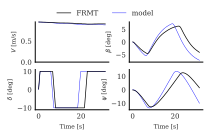
\includegraphics{figures/results_wPCC_ID.closed loop zigzag 10_10 port.pdf}
        \caption{Simulations wPCC Zigzag10/10 to port.}
        \label{fig:sim_wPCC_10}
     \end{subfigure}
     \vfill
     \begin{subfigure}[b]{\textwidth}
        \centering
        \includesvg{figures/results_wPCC_ID.closed loop zigzag 20_20 stbd.svg}
        \caption{Simulations wPCC Zigzag20/20 to starboard.}
        \label{fig:sim_wPCC_20}
     \end{subfigure}
        \caption{Comparison between zigzag tests with wPCC from experiments and simulations with a model equipped with either a polynomial rudder or semi-empirical rudder model.}
        \label{fig:sim_wPCC}
\end{figure}
%\begin{figure}[h]
%     \centering
%     \begin{subfigure}[b]{\textwidth}
%         \centering
%         \includesvg{figures/results_wPCC_ID.overshoot1.svg}
%        \caption{First overshoot angles.}
%        \label{fig:overhoots1_wPCC}
%     \end{subfigure}
%     \vfill
%     \begin{subfigure}[b]{\textwidth}
%         \centering
%         \includesvg{figures/results_wPCC_ID.overshoot2.svg}
%        \caption{Second overshoot angles.}
%        \label{fig:overhoots2_wPCC}
%     \end{subfigure}
%     
%        \caption{Overshoot angles from the wPCC experiments and simulations.}
%        \label{fig:overshoots_wPCC}
%\end{figure}
\FloatBarrier

\subsection{VCT Optiwise}
\noindent A series of fast VCTs with test scenarios as listed in \autoref{tab:VCT_optiwise} were conducted with CFD in Shipflow. Rudder force predictions with the MMG original rudder model and the modified MMG quadratic model were compared to VCT data for the rudder angle variation as shown in \autoref{fig:rudder_angle_compare_optiwise}. The newly added initial inflow angle parameter $\gamma_0$ (see \autoref{eq:gamma_R2}) allows the MMG quadratic model to be better adapted to the VCT data. However, the difference between the models is less obvious when looking at the thrust variation tests in \autoref{fig:rudder_angle_compare_optiwise_all}.

The results of the drift, circle tests and the circle and drift tests are used to validate the MMG model improved by this study (named the MMG quadratic) for the prediction of the rudder forces.
The newly added quadratic relationship for the flow straightening coefficient $\gamma_R$ (\autoref{eq:gamma_R2}) in the MMG quadratic rudder model fits better to the VCT data than the original MMG rudder model, as shown in \autoref{fig:MMG_quadratic}.

%gamma_0, thrust_variation
\begin{figure}[h]
     \centering
     \begin{subfigure}[b]{0.49\textwidth}
         \centering
         \includesvg{figures/results_optiwise_VCT.rudder_angle.svg}
        \caption{Rudder angle variation.}
        \label{fig:rudder_angle_compare_optiwise}
     \end{subfigure}
     \hfill
     \begin{subfigure}[b]{0.49\textwidth}
         \centering
         \includesvg{figures/results_optiwise_VCT.thrust_variation.svg}
        \caption{Thrust variation at \textpm 10 degrees rudder angle.}
        \label{fig:thrust_variation_optiwise}
     \end{subfigure}
    \caption{Rudder angle variation and thrust variation.}
    \label{fig:rudder_angle_compare_optiwise_all}
\end{figure}


%beta_R
\begin{figure}[h]
     \centering
     \begin{subfigure}[b]{0.49\textwidth}
         \centering
         \includesvg{figures/results_optiwise_VCT.Y_R_MMG_original.svg}
        \caption{Original MMG rudder model.}
        \label{fig:Y_R_MMG_original}
     \end{subfigure}
     \hfill
     \begin{subfigure}[b]{0.49\textwidth}
         \centering
         \includesvg{figures/results_optiwise_VCT.Y_R_MMG_quadratic.svg}
        \caption{Modified quadratic MMG rudder model.}
        \label{fig:Y_R_MMG_quadratic}
     \end{subfigure}
    \caption{Rudder force during the VCT tests as a function of the effective inflow angle for the original MMG model and the modified quadratic MMG model.}
    \label{fig:MMG_quadratic}
\end{figure}

The side force generated both on the rudder and the hull surface during various VCT analyses as listed in Table \ref{tab:VCT_optiwise} were used to validate the identified maneuvering model by the proposed procedure for the Optiwise as in \autoref{fig:VCT_optiwise}. The results of the side forces for various rudder angle tests are presented in \autoref{fig:rudder_angle_X_optiwise} -- \autoref{fig:rudder_angle_N_optiwise}, where all the forces are well predicted by the model through the rudder hull interaction coefficients $x_R$ and $a_R$. 
The model predicts zero rudder drag when the rudder angle is zero at straight ahead condition as shown in \autoref{fig:rudder_angle_X_optiwise}. This is because the MMG rudder model has no base drag coefficient like the semi-empirical rudder model for the wPCC (see \autoref{fig:drift_angle_X_wPCC}).
Similar comparisons are shown for the drift angle tests in \autoref{fig:drift_angle_X_optiwise} -- \autoref{fig:drift_angle_N_optiwise} and the circle tests in \autoref{fig:circle_X_optiwise} -- \autoref{fig:circle_N_optiwise}. 


\begin{figure}[h]
    \centering
    %Rudder angle
    \begin{subfigure}[b]{0.325\textwidth}
         \centering
         \includesvg[width=1.2 in]{figures/results_optiwise_VCT.rudder_angle_X.svg}
        \caption{X for Rudder angle tests}
        \label{fig:rudder_angle_X_optiwise}
    \end{subfigure}
    \hfill
    \begin{subfigure}[b]{0.325\textwidth}
        \centering
        \includesvg{figures/results_optiwise_VCT.rudder_angle_Y.svg}
       \caption{Y for Rudder angle tests}
       \label{fig:rudder_angle_Y_optiwise}
    \end{subfigure}
    \hfill
    \begin{subfigure}[b]{0.325\textwidth}
        \centering
        \includesvg{figures/results_optiwise_VCT.rudder_angle_N.svg}
       \caption{N for Rudder angle tests}
       \label{fig:rudder_angle_N_optiwise}
    \end{subfigure}

    \vfill
    %Drift angle
    \begin{subfigure}[b]{0.325\textwidth}
        \centering
        \includesvg{figures/results_optiwise_VCT.drift_angle_X.svg}
       \caption{X for Drift angle tests}
       \label{fig:drift_angle_X_optiwise}
    \end{subfigure}
    \hfill
    \begin{subfigure}[b]{0.325\textwidth}
        \centering
        \includesvg{figures/results_optiwise_VCT.drift_angle_Y.svg}
       \caption{Y for Drift angle tests}
       \label{fig:drift_angle_Y_optiwise}
    \end{subfigure}
    \hfill
    \begin{subfigure}[b]{0.325\textwidth}
        \centering
        \includesvg{figures/results_optiwise_VCT.drift_angle_N.svg}
       \caption{N for Drift angle tests}
       \label{fig:drift_angle_N_optiwise}
    \end{subfigure}
    
    \vfill
    %Circle
    \begin{subfigure}[b]{0.325\textwidth}
        \centering
        \includesvg{figures/results_optiwise_VCT.circle_X.svg}
       \caption{X for Circle tests}
       \label{fig:circle_X_optiwise}
    \end{subfigure}
    \hfill
    \begin{subfigure}[b]{0.325\textwidth}
        \centering
        \includesvg{figures/results_optiwise_VCT.circle_Y.svg}
       \caption{Y for Circle tests}
       \label{fig:circle_Y_optiwise}
    \end{subfigure}
    \hfill
    \begin{subfigure}[b]{0.325\textwidth}
        \centering
        \includesvg{figures/results_optiwise_VCT.circle_N.svg}
       \caption{N for Circle tests}
       \label{fig:circle_N_optiwise}
    \end{subfigure}
    
    \caption{Forces on the Optiwise analyzed by VCT (dots) and predictions from the identified model (lines).}
    \label{fig:VCT_optiwise}
\end{figure}

It should also be noted that the coupling terms $Y_{vrr}$,$Y_{vvr}$,$N_{vrr}$, and $N_{vvr}$ play an important role in accurately modeling the forces. As shown in \autoref{fig:circle_drift_optiwise}, by considering those coupling terms, the sway forces and yaw moments obtained from the identified model give better results than no-coupling models for those circle and drift captive tests.

\begin{figure}[ht]
    \centering
    \includegraphics[width=0.8\linewidth]{figures/results_optiwise_vct.YNH.png}
    \caption{Optiwise hull forces during the circle and drift variations with/without the coupling terms, VCT (dots), fitted model (surface).}
    \label{fig:circle_drift_optiwise}
\end{figure}


% % Circle + drift
% \begin{figure}[h]
%      \centering
%      \begin{subfigure}[b]{0.49\textwidth}
%          \centering
%          \includesvg{figures/results_optiwise_VCT.Y_H.svg}
%         \caption{Sway force.}
%         \label{fig:circle_drift_Y_H_optiwise}
%      \end{subfigure}
%      \hfill
%      \begin{subfigure}[b]{0.49\textwidth}
%          \centering         \includesvg{figures/results_optiwise_VCT.Y_H_no_coupling.svg}
%         \caption{Sway force no coupling.}
%         \label{fig:circle_drift_Y_H_no_coupling_optiwise}
%      \end{subfigure}
     
%      \vfill
%      \begin{subfigure}[b]{0.49\textwidth}
%          \centering
%          \includesvg{figures/results_optiwise_VCT.N_H.svg}
%         \caption{Yawing moment.}
%         \label{fig:circle_drift_N_H_optiwise}
%      \end{subfigure}
%      \hfill
%      \begin{subfigure}[b]{0.49\textwidth}
%          \centering
%          \includesvg{figures/results_optiwise_VCT.N_H_no_coupling.svg}
%         \caption{Yawing moment no coupling.}
%         \label{fig:circle_drift_N_H_no_coupling_optiwise}
%      \end{subfigure}
     
%     \caption{Optiwise hull forces during the circle and drift variations with/without the coupling terms, VCT (dots), fitted model (surface).}
%     \label{fig:circle_drift_optiwise}
% \end{figure}
\FloatBarrier

\subsection{Inverse dynamics analysis Optiwise}
The rudder model within the Optiwise simulation model was replaced by the actual measured rudder forces during the experiments. There was generally good agreement between predictions with the measured rudder model and the corresponding inverse dynamics forces for the zigzag10/10 (\autoref{fig:ID_measured_rudder_zigzag_10_10}) and zigzag20/20 (\autoref{fig:ID_measured_rudder_zigzag_20_20}).
Deviations were however observed for the sway force $Y_D$ during about 3 seconds after the rudder changes at t=11--14 s, and t=35--38 s, for the zigzag10/10 and t=11--14 s, t=35--38 s, t=64 s, for the zigzag20/20. The model and state VCT calculations predict a more straight line in the $Y_D$ time series around these deviation points. 
A reasonable explanation to these deviations has not been found during the work for this paper, where filtration errors in the EKF were ruled out as a possible explanation, by conducting alternative analysis with a low-pass filter instead of the EKF. Accelerations were instead calculated with numeric differentiation of the low-pass filtered signals of repeated zigzag10/10 tests as shown in \autoref{fig:lowpass_deviation_points}.
\begin{figure}[h]
    \centering
    \begin{subfigure}[b]{\textwidth}
        \centering
        \includesvg{figures/results_optiwise_ID.measured_rudder_zigzag 10_10.svg}
        \caption{Zigzag10/10 to port.}
        \label{fig:ID_measured_rudder_zigzag_10_10}
    \end{subfigure}
     \vfill
    \begin{subfigure}[b]{\textwidth}
        \centering
        \includesvg{figures/results_optiwise_ID.measured_rudder_zigzag 20_20.svg}
        \caption{Zigzag20/20 to starboard.}
        \label{fig:ID_measured_rudder_zigzag_20_20}
    \end{subfigure}
    \caption{Inverse dynamics forces during the zigzag tests compared to predictions with the measured rudder model.}
    \label{fig:ID_optiwise20}
\end{figure}
\begin{figure}[h]
    \centering
    \includesvg{figures/results_optiwise_deviation_points.lowpass.svg}
    \caption{Inverse dynamics sway force from repeated zigzag10/10 test to port. The accelerations have been estimated with the EKF and also with numeric differentiation of low-pass filtered signals.}
    \label{fig:lowpass_deviation_points}
\end{figure}

Given the good results with the measured rudder model, focus was on finding a good rudder force prediction model for Optiwise. The MMG original model and the MMG quadratic model -- proposed in this paper -- where fitted to the rudder forces from the VCT data. These models predicted similar forces during the zigzag tests which agreed quite well with the measured forces, especially for the zigzag20/20 test, as shown in \autoref{fig:ID_measured_rudder_zigzag_10_10} and \autoref{fig:ID_measured_rudder_zigzag_20_20}.
\begin{figure}[h]
    \centering
    \begin{subfigure}[b]{\textwidth}
        \centering
        \includesvg{figures/results_optiwise_ID.rudder_forces_zigzag 10_10.svg}
        \caption{Zigzag10/10 to port.}
        \label{fig:ID_measured_rudder_zigzag_10_10}
    \end{subfigure}
     \vfill
    \begin{subfigure}[b]{\textwidth}
        \centering
        \includesvg{figures/results_optiwise_ID.rudder_forces_zigzag 20_20.svg}
        \caption{Zigzag20/20 to starboard.}
        \label{fig:ID_measured_rudder_zigzag_20_20}
    \end{subfigure}
    \caption{Rudder forces during the zigzag tests compared to predictions with the MMG models.}
    \label{fig:ID_optiwise20}
\end{figure}

Similar agreement achieved by the measured rudder model could now be achieved by the models equipped with MMG rudder models, as shown in \autoref{fig:ID_optiwise20}.
\begin{figure}[h]
    \centering
    \begin{subfigure}[b]{\textwidth}
        \centering
        \includesvg{figures/results_optiwise_ID.zigzag 10_10.svg}
        \caption{Zigzag10/10 to port.}
        \label{fig:ID_measured_rudder_zigzag_10_10}
    \end{subfigure}
     \vfill
    \begin{subfigure}[b]{\textwidth}
        \centering
        \includesvg{figures/results_optiwise_ID.zigzag 20_20.svg}
        \caption{Zigzag20/20 to starboard.}
        \label{fig:ID_measured_rudder_zigzag_20_20}
    \end{subfigure}
    \caption{Inverse dynamics forces during the zigzag tests compared to predictions with the MMG models.}
    \label{fig:ID_optiwise20}
\end{figure}



\FloatBarrier
\subsection{Closed loop simulations Optiwise}
Results from closed loop simulations with Optiwise are shown in \autoref{fig:sim_optiwise}. 
\begin{figure}[h]
     \centering
     \begin{subfigure}[b]{0.40\textwidth}
         \centering
         \includesvg{figures/results_optiwise_ID.closed loop zigzag 10_10 port.svg}
        \caption{Zigzag10/10 to port.}
        \label{fig:sim_optiwise_10_port}
     \end{subfigure}
     \hfill
     \begin{subfigure}[b]{0.40\textwidth}
         \includesvg{figures/results_optiwise_ID.closed loop zigzag 10_10 stbd.svg}
        \caption{Zigzag10/10 to starboard.}
        \label{fig:sim_optiwise_10_stbd}
     \end{subfigure}
     \vfill
     \begin{subfigure}[b]{0.40\textwidth}
         \centering
         \includesvg{figures/results_optiwise_ID.closed loop zigzag 20_20 port.svg}
        \caption{Zigzag20/20 to port.}
        \label{fig:sim_optiwise_20_port}
     \end{subfigure}
     \hfill
     \begin{subfigure}[b]{0.40\textwidth}
         \includesvg{figures/results_optiwise_ID.closed loop zigzag 20_20 stbd.svg}
        \caption{Zigzag20/20 to starboard.}
        \label{fig:sim_optiwise_20_stbd}
     \end{subfigure}
     
        \caption{Comparison between zigzag tests with Optiwise from experiments and simulations with a model equipped with either a polynomial rudder or semi-empirical rudder model.}
        \label{fig:sim_optiwise}
\end{figure}

\begin{figure}[h]
     \centering
     \begin{subfigure}[b]{\textwidth}
         \centering
         \includesvg{figures/results_optiwise_ID.overshoot1.svg}
        \caption{First overshoot angles.}
        \label{fig:overhoots1_optiwise}
     \end{subfigure}
     \vfill
     \begin{subfigure}[b]{\textwidth}
         \centering
         \includesvg{figures/results_optiwise_ID.overshoot2.svg}
        \caption{Second overshoot angles.}
        \label{fig:overhoots2_optiwise}
     \end{subfigure}
     
        \caption{Comparison between zigzag tests with Optiwise from experiments and simulations with a model equipped with either a polynomial rudder or semi-empirical rudder model.}
        \label{fig:sim_optiwise}
\end{figure}
\FloatBarrier

\subsection{Rudder inflow analysis Optiwise}
The rudder inflow angle $\gamma$ and velocity $V_R$ were investigated by conducting a set of separate VCT calculations where the rudder was removed, so that an undisturbed flow by the rudder could be observed. The longitudinal and transverse inflow velocities $u_R$ and $v_R$ were measured along the rudder stock from the root to the tip of the rudder. \autoref{fig:rudder_velocities_span} shows the inflow velocity $\gamma=atan(v_R/u_R)$ along the rudder stock during two circle tests.
\begin{figure}[h]
    \centering 
    \includesvg{figures/results_optiwise_rudder_velocities.span_circle.svg}
    \caption{Rudder inflow angle from the root to the tip of the rudder during two circle tests.}
     \label{fig:rudder_velocities_span}
\end{figure}
\begin{figure}[h]
     \centering
     \begin{subfigure}[b]{\textwidth}
         \centering
         \includesvg{figures/results_optiwise_rudder_velocities.drift_angle.svg}
        \caption{Drift angle.}
        \label{fig:inflow_to_force_drift_angle}
     \end{subfigure}
     \vfill
     \begin{subfigure}[b]{\textwidth}
         \includesvg{figures/results_optiwise_rudder_velocities.circle.svg}
        \caption{Circles.}
        \label{fig:inflow_to_force_circle}
     \end{subfigure}
        \caption{Rudder forces from VCT and predictions from the measured inflow velocities.}
        \label{fig:inflow_to_rudder_force}
\end{figure}

\FloatBarrier

%%%%%%%%%%%%%%%
%% DISCUSSION
%%%%%%%%%%%%%%%
\section{Discussion}
\label{sec:discussion}

%%%%%%%%%%%%%%%
%% CONCLUSIONS
%%%%%%%%%%%%%%%
\section{Conclusions}
\label{sec:conclusions}
%_________________________________________________________
%Move 1: Background information (research purposes, theory,
%methodology)
%
%The objective of this paper was to investigate if the PI model is physically more correct than a physics uninformed model (PU model), when they are both identified from zigzag model tests, and also to investigate how this affects the generalization.

%_________________________________________________________
%Move 2: Summarizing and reporting key results. (oblig.)

%_________________________________________________________
%Move 3: Commenting on key results (making claims, explaining the results,
%comparing the new work with previous studies, offering
%alternative explanations) (oblig.)

%_________________________________________________________
%Move 4: Stating the limitations of the study

%_________________________________________________________
%Move 5: Making recommendations for future implementation and/or for
%future research

\FloatBarrier

\section{Acknowledgements}
\input{acknowledgements}

%% The Appendices part is started with the command \appendix;
%% appendix sections are then done as normal sections
\appendix


\FloatBarrier
%% If you have bibdatabase file and want bibtex to generate the
%% bibitems, please use
%%
\pagebreak
\bibliographystyle{elsarticle-harv}
%\bibliography{Paper_3_semiempirical_rudder.bib}
\bibliography{Paper_5.bib}

\end{document}

\endinput
%%
%% End of file `elsarticle-template-harv.tex'.
